%%%%%%%%%%%%%%%%%%%% author.tex %%%%%%%%%%%%%%%%%%%%%%%%%%%%%%%%%%%
%
% sample root file for your "contribution" to a contributed volume
%
% Use this file as a template for your own input.
%
%%%%%%%%%%%%%%%% Springer %%%%%%%%%%%%%%%%%%%%%%%%%%%%%%%%%%


% RECOMMENDED %%%%%%%%%%%%%%%%%%%%%%%%%%%%%%%%%%%%%%%%%%%%%%%%%%%
\documentclass[graybox]{svmult}

% choose options for [] as required from the list
% in the Reference Guide

\usepackage{type1cm}        % activate if the above 3 fonts are
                            % not available on your system
%
\usepackage{makeidx}         % allows index generation
\usepackage{graphicx}        % standard LaTeX graphics tool
                             % when including figure files
\usepackage{multicol}        % used for the two-column index
\usepackage[bottom]{footmisc}% places footnotes at page bottom


\usepackage{newtxtext}       % 
\usepackage{newtxmath}       % selects Times Roman as basic font

% see the list of further useful packages
% in the Reference Guide

\makeindex             % used for the subject index
                       % please use the style svind.ist with
                       % your makeindex program

%%%%%%%%%%%%%%%%%%%%%%%%%%%%%%%%%%%%%%%%%%%%%%%%%%%%%%%%%%%%%%%%%%%%%%%%%%%%%%%%%%%%%%%%%

%Useful examples:     I didnt wanna just delete the some templates because we might need to use them later.

%\footnote{If you copy text passages, figures, or tables from other works, you must obtain \textit{permission} from the copyright holder (usually the original publisher). Please enclose the signed permission with the manuscript. The sources\index{permission to print} must be acknowledged either in the captions, as footnotes or in a separate section of the book.}
%\textit{tilted word}

%\begin{quotation}
% Please do not use quotation marks when quoting texts! Simply use the \verb|quotation| environment -- it will automatically be rendered in line with the preferred layout.
%\end{quotation}

% \LaTeX\ 
% \ref{sec:2}.





\begin{document}

\title*{Drag reduction from different of shark denticles}
% Use \titlerunning{Short Title} for an abbreviated version of
% your contribution title if the original one is too long
\author{Gökçe Atacan and Akash Tejveer Dwarka}
% Use \authorrunning{Short Title} for an abbreviated version of
% your contribution title if the original one is too long
\institute{Gökçe Atacan \at Lycoming College, Pennsylvania, \email{atagokc@lycoming.edu}
\and Akash Tejveer Dwarka \at Lycoming College, Pennsylvania \email{dwaakas@lycoming.edu}}
%
% Use the package "url.sty" to avoid
% problems with special characters
% used in your e-mail or web address
%
\maketitle


\abstract{Each chapter should be preceded by an abstract (no more than 200 words) that summarizes the content.}

\section{Introduction}
\label{sec:1}

Whether it is through air or water, reducing a body's resistive forces is usually one of the goals while designing a vehicle. The majority of the resistive force is drag. In fact, it is so relevant with trading ships that it contributes to around 70\% of the resistive forces \cite{lindholdt_effects_2015}. Reducing this figure would cause a trickle-down effects to shipping and transport costs. 

Reif among others have established at least four decades ago that shark skins can reduce drag \cite{reif_morphogenesis_1982}. These are shark denticles: tiny scale-like structures that prevent fluids from detaching from their surface. These structures are on the submillimeter scale that seems to reduce drag by up to 9.9\% \cite{bechert_experiments_1997}. However, further experiments showed drag reduction of up to 25.4\% \cite{guo_experimental_2023}.

While experiments have shown how shark denticles reduce drag, there are also theories that suggest how they do so. Near the surface of the skin, the fluid flowing along mean velocity stays attached. However, the fluid might get detached an flow along the perpendicular direction \cite{bechert_experiments_1997}. The shark denticles have riblets that stops these perpendicular components and rectify the fluid along the mean velocity keeping the flow attached \cite{guo_experimental_2023}. This then reduces shear-stresses and reduces drag.

Most experiments and simulations, however, simplify the denticles that simple grooves. While there were effort to replicate denticles as a three-dimensional structure, they base themselves on one species of shark: \textit{Isurus oxyrinchus}. Despite being the fastest shark, there is merit to studying other species' denticles \cite{graybill_experimental_2024}.

By referring to Scanning Electron Microscope (SEM) and micro-CT scan models of denticles from different shark species, we created denticles models for shortfin mako (\textit{Isurus oxyrinchus}), smooth dogfish sharks (\textit{Mustelus canis}), blacktip shark (\textit{Carcharhinus limbatus}), and White shark (\textit{Carcharodon carcharias}) \cite{ankhelyi_diversity_2018}. We created the models using the measurements of key features such as the crown length, crown width, riblet spacing, and ridge depth.

We then compared the drag reduction ($\nu$) by simulation the fluid flow using the $k\omega$-SST model at different fluid speeds. We placed a row of denticles on a NACA0012 airfoil. We then created a generic shark model and placed the denticles on its fins, tails and snout to determine whether the type of denticles causes significant reduction in drag.

\section{Related Work and Background}
\label{sec:2}

\textbf{Title} This is how they did it

How is the mechanism helpful in turbulent flow (READ https://royalsocietypublishing.org/rsif/article/15/147/20180473/35940/Passive-bristling-of-mako-shark-scales-in)

Explain different experiments. CITES

Explain different simulations

Difficulties with experiments and scales CITE-REVIEW
(Recreation methods by Zhang et al.)

Refer previous drag reduction values CITES
MAKE TABLE

Refer to paper with denticle measurements
MAKE TABLE

\section{Data and Methodology}
\label{sec:3}
% Always give a unique label
% and use \ref{<label>} for cross-references
% and \cite{<label>} for bibliographic references
% use \sectionmark{}
% to alter or adjust the section heading in the running head
Please include a brief intro for your process of gathering data, which methods you used, and/or why you chose these datasets and methods.

Fusion 360,cripting, openfoam -simulation properties, paraview, some calculation, some comparison and some graphs here.
Dahası var mı yoksa yine mi compile etmem lazım????"

In this research we did numerical experiments with openfoam to get rid of scaling problem that most of the experiments are facing because of the manufacturing limits.
Also, we designed the denticles inspirated from [idk some resource] on fusion 360. Also we parametrized the design by scripting the denticles models to control the parameters better. 
Also, if anyone wants to replicate this paper, they are welcome to use the script to create the denticle models.
Pictures of denticles with the name of the sharks and tehnical drawings of them.

Then, we ran the simulations exactly with the exactly same parameters to this paper [cite the paper.] on OpenFoam
The openFoam folders will be available.
!Mention that we scaled the denticles same with the paper because their denticle size is about 60 times bigger. [cite the paper]
Some formulas to show how we calculated the drag coefficient, etc. 
Then redo the simulation with actual denticle size. --Maybe we might need to change the angle of attack to be able see the drag better. Detect the best angle from the paper for drag reduction

We replaced it with other type of denticles and compare the results between denticles. 


\subsection{Data Collection --Maybe we should change the name???}
\label{subsec:2}

General description of what is coming- simulation properties and how did we set up paraview.
We have data of smooth airfoil (airfoil without denticle), scenario a for [cite paper here] which is a row of denticles located at the L= (id remember the val) on NACA 0012 airfoil with 0 degree angle of attack. 
We will have more data. Coming...


\subsubsection{Simulation Setup}
\label{subsec:3}
All tecnical drawing of denticle 

Measurement of airfoil 

Properties of simulation and turbulence, solver etc.


\subsubsection{Postprocessing}
\label{subsec:4}
Talk about how to make calculation or how to use paraview etc. 

%\begin{figure}[ht]
%  \centering
%  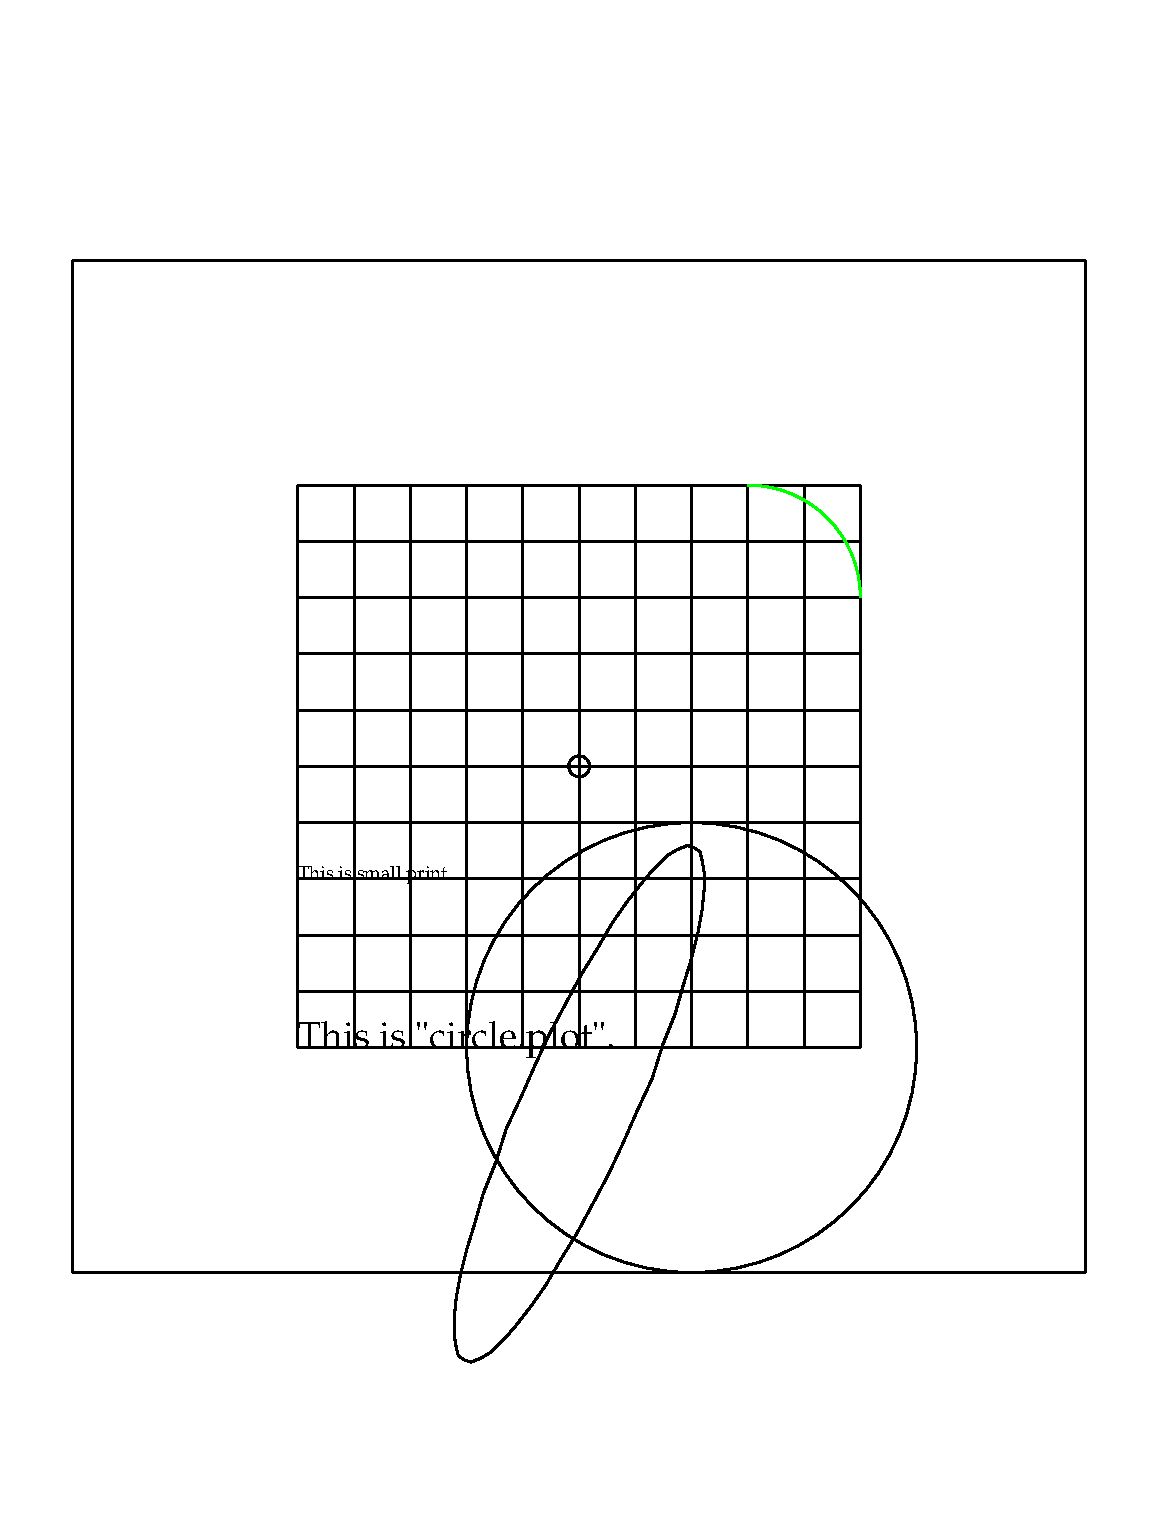
\includegraphics[width=.7\textwidth]{figure}
%  \caption{Figures should always have a caption.}
%  \label{fig:1}
%\end{figure}


\subsection{Experiment or Methods or idk}
\label{subsec:5}

Tamam simulasyon falan hazır da nereye konumlandırdın denticleları ya da koyduğun geometriyi nasıl kombinasyonlarda koydun. 


\subsubsection{Method Subsection 1}
sth sth sth --We might not need this one.


\section{Results}
\label{sec:4}
% Always give a unique label
% and use \ref{<label>} for cross-references
% and \cite{<label>} for bibliographic references
% use \sectionmark{}
% to alter or adjust the section heading in the running head
Provide a description of main findings in chronological order of the data represented in the methods section. Include a summary of research findings. Repeat questions to help readers understand results. Additionally, include a report about information collection, participants, and recruitment.

Show data presented in tables, charts, graphs, and other figures.

Put graphs or picture from the replicated scenario of the reference paper. 
Put numbers of results
Put numbers of comparison 
Compare and make comments 


 
\subsection{Validation of simulation}


Here will be comparison of the replicated simulation and the reference paper. 

\subsection{Comparison of across denticles}

Here will be comparison of different denticle models.

\section{Conclusion}
\label{sec:5}
% Always give a unique label
% and use \ref{<label>} for cross-references
% and \cite{<label>} for bibliographic references
% use \sectionmark{}
% to alter or adjust the section heading in the running head
Conclusion will be addeed later. 

\subsection{Applications} %
Application fields will be added later.

\subsection{Concerns and Future Work} %
Concerns and future work will be added later. s


\begin{acknowledgement}
We can add an acknowledgement, thank you for Teuscher lab and opportunity that they provided us to have remote research etc. etc.

  If you want to include acknowledgments of assistance and the like at the end of an individual chapter please use the \verb|acknowledgement| environment -- it will automatically be rendered in line with the preferred layout.
\end{acknowledgement}



% Bibliography
\bibliography{denticles} 
\bibliographystyle{plain}



\end{document}
